\chapter{Unsupervised Learning in Recurrent Networks}\label{ch_unsupervised_recurrent}
\chapterauthor{Jeff Yoshimi}

% Add IAC somewhere? It is the initial motivating example and the underlying idea is in the background here, though in IAC a but more dynamic emphasis as we settle into things. The "answers" are attractors. The transients have meaning. Spivey and JTrace people do work on this. 

\section{Introduction}

In this chapter we consider recurrent networks trained using the Hebb rule to complete patterns. This continues the discussion of unsupervised learning in feed-forward pattern associators that began in chapter \extref{ch_unsupervised}, but applies those ideas to networks that associate fragments of patterns will full patterns. We will see that the tools of dynamical systems theory (chapter \extref{ch_dst}) are quite useful in this context. In chapter \extref{ch_supervised_recurrent} we discuss more complex recurrent networks and their applications to psychology, neuroscience, and engineering.
  
\section{Hebbian Pattern Association for Recurrent Networks}

We now consider a \emph{recurrent} network trained using the Hebb law. When the Hebb rule is used in a recurrent network, nodes can be trained to co-activate one another. These co-activations will cascade through the network, strengthening connections between co-active nodes, and the result will be a kind of trace of whatever pattern was used to train the network. When a partial cue is used later, the entire pattern will be recreated. An example that makes the idea clear is in Fig. \ref{patternCompletionL}, where the residue of past training on an ``L''-shaped pattern (a ``memory trace'') is evident. When the network is updated, it is obvious that the activation will fill in the L-shape. 

Because they associate part of pattern with the whole pattern, these networks are sometimes thought of as auto-associators.
% Link to ff auto-associator; really kind of a separate category

\begin{figure}[h]
\centering
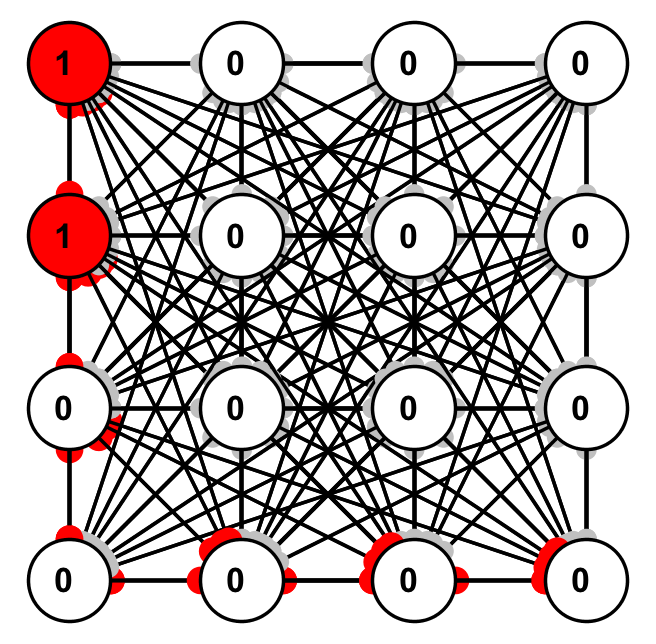
\includegraphics[scale=.5]{./images/patternCompletion_Cue}
\caption[Simbrain screenshot.]{Cued recall of an ``L'' shaped pattern. Notice that the ``L'' pattern is visible in the red weights, which indicate how the pattern will be completed. In the past, those neurons fired together, so they were wired together by the Hebb rule.}
\label{patternCompletionL}
\end{figure}

% Citation to scientific literature below.
These ideas can be used to explain visual image completion. When we see a fragment of a familiar image or visual scene, we can often ``fill in the rest''. This can be understood in terms of trained associations in a recurrent network where each node corresponds to a pixel in an image. When a pattern is learned all the correlations between pixels are encoded by strengthening the connections between those neurons using the Hebb rule. An example of a recurrent auto-associator for visual memories is shown in Fig. \ref{patternCompletionBeerDog}. It's the same idea as with the simple ``L'' pattern in Fig. \ref{patternCompletionL}, but with a much larger network, containing half a million rather a few hundred weights. In each case learning a memory amounts to strengthening co-active nodes in a grid of nodes. In both cases a partial cue triggers the completion of a stored pattern. The formation and recall of visual memories, and perhaps certain features of imagination, can be understood in these terms. 
%\footnote{The small network has $(4 \cdot 4) = 16$ nodes, and thus $16^2 = 256$ weights; the larger network has $(130 \cdot 180) = 23,400$ nodes and thus $23,400^2 = 547,560,000$ weights.} <- Check these numbers. The small net does not self connections, not sure about the larger one

\begin{figure}[h]
\centering
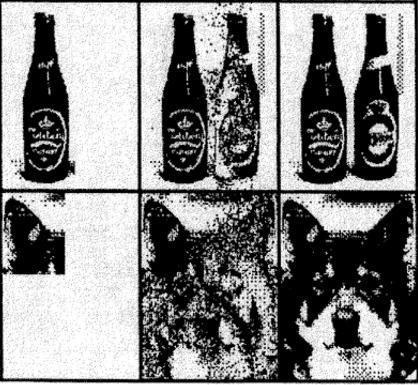
\includegraphics[scale=.8]{./images/patternCompletionBeerDog.png}
\caption[From Hertz, Krogh, and Palmer, 1991 \cite{hertz1991introduction}.]{Pattern completion in a recurrent network with $130 \cdot 180 = 23,400$ nodes. The left-most image in each row shows the initial cue. The middle image shows the network part-way through the pattern completion process. The right image shows the final image. From Hertz et al. 1991. The network is a Hopfield network, which uses a variant on the Hebb rule.}
\label{patternCompletionBeerDog}
\end{figure}


\begin{figure}[h]
\centering
\frame{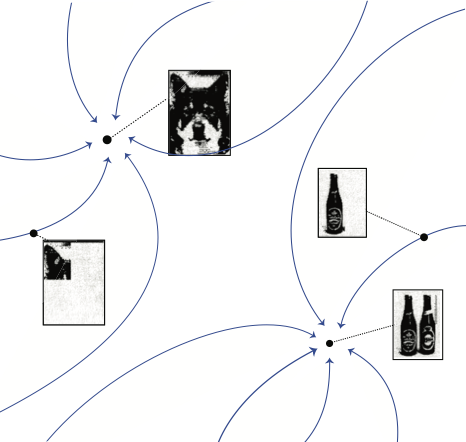
\includegraphics[scale=.5]{./images/attractorsBeerDog.png}}
\caption[Pamela Payne, using elements from Hertz, Krogh, and Palmer, 1991 \cite{hertz1991introduction}.]{Schematic diagram of the attractors and basins of attraction for the images shown in Fig. \ref{patternCompletionBeerDog}. Fragments of images correspond to initial conditions, that evolve under the network dynamics to completed images, which correspond to attracting fixed points.}
\label{beerDogAttractors}
\end{figure}
The nice thing about taking this approach is that we can use it to study some very simple examples that we can run by hand, like with the simple feed-forward associators discussed in \extref{ch_unsupervised}. For practice, try using the self-contained Simbrain workspace simulations / tutorials \emph{autoAssociatorPart1.zip} and \emph{autoAssociatorPart2.zip}, created by Alex Holcombe. 

% Reinforce the links below with a bulleted list (see learning objectives). Also add oscillations -> n-cycles.
Figure \ref{beerDogAttractors} shows how pattern completion in recurrent auto-associators can be understood in terms of   dynamical systems theory (also see chapter \extref{ch_dst}). Each new pattern the network is trained on becomes a fixed point attractor in its activation space. The beer and dog images on the right of Fig. \ref{patternCompletionBeerDog} are fixed point attractors in the 23,400-dimensional activation space of that network. The ``L'' visible as a trace in Fig. \ref{patternCompletionL} is a fixed point attractor of the 16-dimensional activation space of that network. A cue corresponds to an initial condition. The single beer bottle and dog's ear in Fig. \ref{patternCompletionBeerDog} are initial conditions, as is the upper part of the ``L'' in Fig. \ref{patternCompletionL}. Recall corresponds to following an orbit through the activation space. The final memory is the attractor corresponding to whatever basin of attraction the initial condition was in. Thus, on this model, learning a new pattern via Hebb's rule corresponds to adding a new attractor to the network's state space.\footnote{Thus learning in these cases also counts as a bifurcation, since this corresponds to a change of parameters (weights) that produces a change in the topological structure of the orbits in the state space.}

% Local representations
%The advantage of thinking about recurrent auto-associators in terms of images is that it's immediately, visually obvious how they work. But recurrent auto-associators can also be understood more abstractly. If we think of each node in an auto-associator as one memory, then we can simply think about an auto-associator as connecting these localist memories together. Such a network, once trained, is a lot like the IAC networks (e.g. the Jets and Sharks model) discussed in chapter \extref{ch_intro}. In such a network attributes of gang members---their job, their name, their age, etc---are recalled when some of those attributes are activated and the network is run. This is exactly what happens in a recurrent auto-associator. But whereas weights in an IAC network are set by hand, the Hebb rule shows how they can be \emph{learned}. You set all the weights to be connected to ``on'' and then apply the rule, and the associations are encoded.

\section{Some features of recurrent auto-associators}

First, they perform fairly well even if some synapses are removed (graceful degradation) or if you add noise to the inputs.

Second, the memories you train them on often interfere with one another. Small networks trained using binary inputs (patterns of 0's and 1's, as in see Figure \ref{binary}) cannot easily learn more than one  memory. If a second pattern overlaps the first (in which case the two input vectors are not orthogonal), then during recall any partial version of either pattern will produce the \emph{conjunction} of the two patterns. This is sometimes called \emph{cross-talk} or \emph{interference}. To address the problem, we can use \emph{bipolar} patterns (see Figures \ref{binary} and \ref{bipolar} to see how binary and bipolar patterns compare), in which the ``off'' neurons are set to -1. The reason this helps is that the network is now learning not only to recreate a pattern of correlated activations, but also to \emph{inhibit} activations inconsistent with the current pattern. The ``on'' nodes are connected to the ``off'' nodes with negative weights. Thus, during recall, activating one pattern will inhibit other patterns. This in turn makes it possible to store overlapping patterns. One pattern simultaneously represses the other. 
% If you store two patterns with just one overlapping unit, for example, you will notice that both can be independently recalled. 

\begin{figure}[h]
\centering
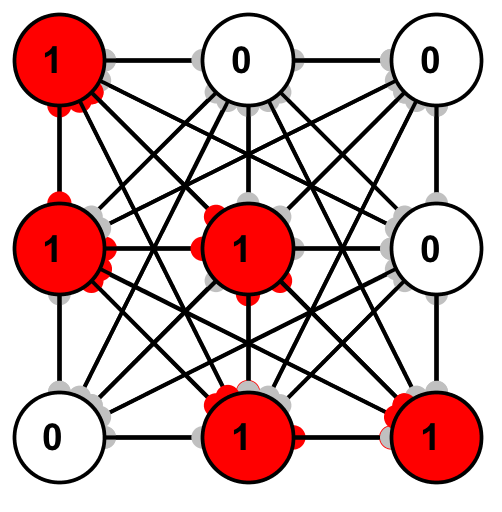
\includegraphics[scale=.6]{./images/hebb_binary_9.png}
\caption[Simbrain screenshot.]{An auto associative network trained on a single pattern using Hebb's rule. Notice that only weights between co-active nodes have been strengthened. Since the other nodes have activations of 0, weights to and from them are not changed.}
\label{binary}
\end{figure}

\begin{figure}[h]
\centering
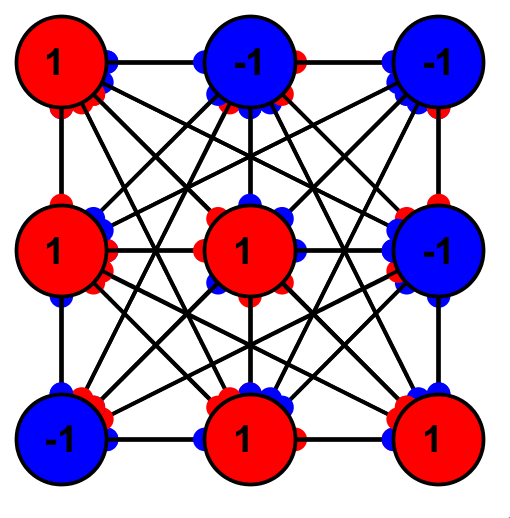
\includegraphics[scale=.6]{./images/hebb_bipolar_9.png}
\caption[Simbrain screenshot]{Bipolar version of pattern from Fig. \ref{binary}, after training on a bipolar version of the same pattern. Notice how some of the weights have turned blue. Thus when the pattern is recreated incompatible patterns will be inhibited. This version of the network can learn several patterns.}
\label{bipolar}
\end{figure}
% Say more. See Hopfield paper. Potential for recall is proportional to hamming error between patterns. Something like that.

% Make more about anti-patterns and this point in general. For assignment.
Third, when you train a recurrent network, you will sometimes notice new patterns, which are byproducts of other patterns: these are sometimes called \emph{spurious memories}. In the case of a network trained on 1 bipolar pattern, these are easy to predict: they correspond to the compliment of the trained pattern (that is, the pattern formed by -1's rather than 1's).\footnote{One way to get a feel for this is to use a projection to see all the stored and spurious patterns, which are attractors of the network. Often these will appear to be symmetrically positioned vertices of a hypercube.} 
% These techniques can be scaled up to networks with more neurons. One experiment you can try is creating a network with 25 neurons, intepreting the nodes as pixels, and then teaching it a few letters of the alphabet.

Fourth, another problem we run into with these networks is oscillations. If you try multiple initial conditions in a recurrent network trained using the Hebb rule, it may sometimes oscillate through an $n$-cycle rather than settling in to a fixed point attractor. In our study of dynamical systems in chapter \extref{ch_dst} we saw that oscillations---i.e. attracting periodic orbits---often appear in recurrent networks. Using the Hebb rule can store a fixed point attractor memory, but un-desired $n$-cycles can come along for the ride. Hopfield networks, discussed next, avoid this problem.

% You can also analyze the network using dynamical systems theory. If you put the network in to random activation states (by selecting all neurons and pressing the randomize button) and iterate, you will note that it either settles into the pattern you created or to its ``dual,'' a pattern of -1's on the same neurons (this is also called a ``spurious'' memory). You can visualize this by opening a projection plot. Any point in activation space will evolve to one of these two attracting fixed points. Thus you have, via learning, created two attractors corresponding to this pattern and its dual.

% In terms of dynamical systems theory, what is happening is that we are observing periodic orbits in the network's activation space. Hopfield networks, discussed next, solve the problem of oscillations, but most of the other problems remain.

\section{Hopfield Networks}

% Reference below. 
A special type of recurrent, auto associative, Hebbian network is a Hopfield network.\footnote{Hopfield networks are important historically. When John Hopfield, a physicist, introduced them in the 1970s it brought the existing engineering literature on neural networks and the formalisms in physics in to greater contact than they had before. Hopfield also pioneered the use of rigorous dynamical systems theory in neural networks \cite{hopfield1982neural}.}  Hopfield networks have no self-connections and their weights are always symmetrical ($w_{i,j} = w_{j,i}$ for every weight in the network). They are also updated in a special way that helps avoid the unwanted oscillations ($n$-cycles where $n>1$).
% Footnote on what asynchronous update is.
% Mention triangular matrices

A Hopfield network with 80 nodes that is treated as a very small pixel display is shown in Fig. \ref{F:hopfield} after it has retrieved one of the 4 memories it was trained on, a memory corresponding to the letter ``Z''.

\begin{figure}[h]
\centering
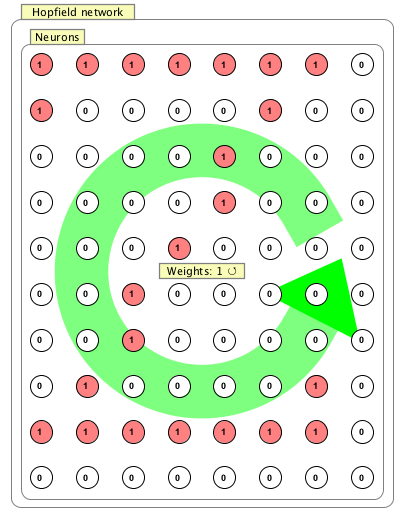
\includegraphics[scale=.4]{./images/Hopfield.png}
\caption[Simbrain screenshot]{Hopfield network trained on the pattern for a ``Z''. Though a binary pattern is displayed behind the scenes this network uses bipolar patterns, with -1's where 0s are.}
\label{F:hopfield}
\end{figure}

% Citation
The memory capacity of Hopfield networks has been estimated to be 15\%  of its number of nodes (see Fausett, p. 140 \cite{fausett1994fundamentals}, Hopfield p. 2556).\footnote{A discussion of storage capacity for associative memories in general is in Fausett, section 3.3.4).}  Thus, a network with 20 nodes should be able to store about $3 = .15 \cdot 20$ memories. Hopfield networks have the advantage of not producing oscillations. However, they do produce spurious memories. To get a feel for how Hopfield networks work, you are encouraged to try the Simbrain simulation \emph{hopfieldNet.zip} or to make and train a Hopfield network from scratch. 
% If you right click on the interaction box for a Hopfield network you will see several commands that make it easy to quickly train a Hopfield network without all the careful clamping and unclamping required in the more generic recurrent networks described above.
